\documentclass[8pt,a4paper]{article}
\usepackage[utf8]{inputenc}
\usepackage{amsmath}
\usepackage{amsfonts}
\usepackage{amssymb}
%My personal maths package
%\bibliography{Bibliography.bib}

%%%%%%%%%%%%%%%%%%%%%%%%%%%%%%%%%%%%%%%%%%%%%%%%%%%%%%%%%%%%%%%%%%%%%%%%%%%%%%
%%%%% MATH PACKAGES %%%%%%%%%%%%%%%%%%%%%%%%%%%%%%%%%%%%%%%%%%%%%%%%%%%%%%%%%%
%%%%%%%%%%%%%%%%%%%%%%%%%%%%%%%%%%%%%%%%%%%%%%%%%%%%%%%%%%%%%%%%%%%%%%%%%%%%%%

% very good package
%\usepackage{mathtools}

%%% font stuff
\usepackage[T1]{fontenc}        % for capitals in section /paragraph etc.
\usepackage[utf8]{inputenc}     % use utf8 symbols in code

\usepackage{amssymb,amsmath,amsfonts} % amsthm not needed -- use my own envs
%\usepackage{mathtools}
%\mathtoolsset{showonlyrefs}
% further alternative math packages: unicode-math, abx-math
\usepackage{bm}
\usepackage{mathrsfs} % used for: fraktal math letters
\usepackage[bigsqcap]{stmaryrd} % used for: big square cap symbol
\usepackage{xargs}

% standard packages
%\usepackage{color} % for color

%%
%%index

\newcommand*{\keyword}[2][\empty]{\emph{#2}\ifx#1\empty\index{#2}\else\index{#1}\fi}
\newcommand*{\person}[1]{\textsc{#1}}

%%%%%%%%%%%%%%%%%%%%%%%%%%%%%%%%%%%%%%%%%%%%%%%%%%%%%%%%%%%%%%%%%%%%%%%%%%%%%%%%%%%%%%%%%%%%%%%%%%%%%%%%%%%%
%%%%% MATH ALPHABETS & SYMBOLS %%%%%%%%%%%%%%%%%%%%%%%%%%%%%%%%%%%%%%%%%%%%%%%%%%%%%%%%%%%%%%%%%%%%%%%%%%%%%
%%%%%%%%%%%%%%%%%%%%%%%%%%%%%%%%%%%%%%%%%%%%%%%%%%%%%%%%%%%%%%%%%%%%%%%%%%%%%%%%%%%%%%%%%%%%%%%%%%%%%%%%%%%%

% w: http://milde.users.sourceforge.net/LUCR/Math/math-font-selection.xhtml

% ===== Set quick commands for math letters ================================================================
% calagraphic letters (only upper case available; standard)
\newcommand{\cA}{\mathcal{A}}
\newcommand{\cB}{\mathcal{B}}
\newcommand{\cC}{\mathcal{C}}
\newcommand{\cD}{\mathcal{D}}
\newcommand{\cE}{\mathcal{E}}
\newcommand{\cF}{\mathcal{F}}
\newcommand{\cG}{\mathcal{G}}
\newcommand{\cH}{\mathcal{H}}
\newcommand{\cI}{\mathcal{I}}
\newcommand{\cJ}{\mathcal{J}}
\newcommand{\cK}{\mathcal{K}}
\newcommand{\cL}{\mathcal{L}}
\newcommand{\cM}{\mathcal{M}}
\newcommand{\cN}{\mathcal{N}}
\newcommand{\cO}{\mathcal{O}}
\newcommand{\cP}{\mathcal{P}}
\newcommand{\cQ}{\mathcal{Q}}
\newcommand{\cR}{\mathcal{R}}
\newcommand{\cS}{\mathcal{S}}
\newcommand{\cT}{\mathcal{T}}
\newcommand{\cU}{\mathcal{U}}
\newcommand{\cV}{\mathcal{V}}
\newcommand{\cW}{\mathcal{W}}
\newcommand{\cX}{\mathcal{X}}
\newcommand{\cY}{\mathcal{Y}}
\newcommand{\cZ}{\mathcal{Z}}

% bold math letters (standard)
\newcommand{\bfA}{\mathbf{A}}
\newcommand{\bfB}{\mathbf{B}}
\newcommand{\bfC}{\mathbf{C}}
\newcommand{\bfD}{\mathbf{D}}
\newcommand{\bfE}{\mathbf{E}}
\newcommand{\bfF}{\mathbf{F}}
\newcommand{\bfG}{\mathbf{G}}
\newcommand{\bfH}{\mathbf{H}}
\newcommand{\bfI}{\mathbf{I}}
\newcommand{\bfJ}{\mathbf{J}}
\newcommand{\bfK}{\mathbf{K}}
\newcommand{\bfL}{\mathbf{L}}
\newcommand{\bfM}{\mathbf{M}}
\newcommand{\bfN}{\mathbf{N}}
\newcommand{\bfO}{\mathbf{O}}
\newcommand{\bfP}{\mathbf{P}}
\newcommand{\bfQ}{\mathbf{Q}}
\newcommand{\bfR}{\mathbf{R}}
\newcommand{\bfS}{\mathbf{S}}
\newcommand{\bfT}{\mathbf{T}}
\newcommand{\bfU}{\mathbf{U}}
\newcommand{\bfV}{\mathbf{V}}
\newcommand{\bfW}{\mathbf{W}}
\newcommand{\bfX}{\mathbf{X}}
\newcommand{\bfY}{\mathbf{Y}}
\newcommand{\bfZ}{\mathbf{Z}}
\newcommand{\bfa}{\mathbf{a}}
\newcommand{\bfb}{\mathbf{b}}
\newcommand{\bfc}{\mathbf{c}}
\newcommand{\bfd}{\mathbf{d}}
\newcommand{\bfe}{\mathbf{e}}
\newcommand{\bff}{\mathbf{f}}
\newcommand{\bfg}{\mathbf{g}}
\newcommand{\bfh}{\mathbf{h}}
\newcommand{\bfi}{\mathbf{i}}
\newcommand{\bfj}{\mathbf{j}}
\newcommand{\bfk}{\mathbf{k}}
\newcommand{\bfl}{\mathbf{l}}
\newcommand{\bfm}{\mathbf{m}}
\newcommand{\bfn}{\mathbf{n}}
\newcommand{\bfo}{\mathbf{o}}
\newcommand{\bfp}{\mathbf{p}}
\newcommand{\bfq}{\mathbf{q}}
\newcommand{\bfr}{\mathbf{r}}
\newcommand{\bfs}{\mathbf{s}}
\newcommand{\bft}{\mathbf{t}}
\newcommand{\bfu}{\mathbf{u}}
\newcommand{\bfv}{\mathbf{v}}
\newcommand{\bfw}{\mathbf{w}}
\newcommand{\bfx}{\mathbf{x}}
\newcommand{\bfy}{\mathbf{y}}
\newcommand{\bfz}{\mathbf{z}}

% fractal math letters (standard)
\newcommand{\fkA}{\mathfrak{A}}
\newcommand{\fkB}{\mathfrak{B}}
\newcommand{\fkC}{\mathfrak{C}}
\newcommand{\fkD}{\mathfrak{D}}
\newcommand{\fkE}{\mathfrak{E}}
\newcommand{\fkF}{\mathfrak{F}}
\newcommand{\fkG}{\mathfrak{G}}
\newcommand{\fkH}{\mathfrak{H}}
\newcommand{\fkI}{\mathfrak{I}}
\newcommand{\fkJ}{\mathfrak{J}}
\newcommand{\fkK}{\mathfrak{K}}
\newcommand{\fkL}{\mathfrak{L}}
\newcommand{\fkM}{\mathfrak{M}}
\newcommand{\fkN}{\mathfrak{N}}
\newcommand{\fkO}{\mathfrak{O}}
\newcommand{\fkP}{\mathfrak{P}}
\newcommand{\fkQ}{\mathfrak{Q}}
\newcommand{\fkR}{\mathfrak{R}}
\newcommand{\fkS}{\mathfrak{S}}
\newcommand{\fkT}{\mathfrak{T}}
\newcommand{\fkU}{\mathfrak{U}}
\newcommand{\fkV}{\mathfrak{V}}
\newcommand{\fkW}{\mathfrak{W}}
\newcommand{\fkX}{\mathfrak{X}}
\newcommand{\fkY}{\mathfrak{Y}}
\newcommand{\fkZ}{\mathfrak{Z}}
\newcommand{\fka}{\mathfrak{a}}
\newcommand{\fkb}{\mathfrak{b}}
\newcommand{\fkc}{\mathfrak{c}}
\newcommand{\fkd}{\mathfrak{d}}
\newcommand{\fke}{\mathfrak{e}}
\newcommand{\fkf}{\mathfrak{f}}
\newcommand{\fkg}{\mathfrak{g}}
\newcommand{\fkh}{\mathfrak{h}}
\newcommand{\fki}{\mathfrak{i}}
\newcommand{\fkj}{\mathfrak{j}}
\newcommand{\fkk}{\mathfrak{k}}
\newcommand{\fkl}{\mathfrak{l}}
\newcommand{\fkm}{\mathfrak{m}}
\newcommand{\fkn}{\mathfrak{n}}
\newcommand{\fko}{\mathfrak{o}}
\newcommand{\fkp}{\mathfrak{p}}
\newcommand{\fkq}{\mathfrak{q}}
\newcommand{\fkr}{\mathfrak{r}}
\newcommand{\fks}{\mathfrak{s}}
\newcommand{\fkt}{\mathfrak{t}}
\newcommand{\fku}{\mathfrak{u}}
\newcommand{\fkv}{\mathfrak{v}}
\newcommand{\fkw}{\mathfrak{w}}
\newcommand{\fkx}{\mathfrak{x}}
\newcommand{\fky}{\mathfrak{y}}
\newcommand{\fkz}{\mathfrak{z}}

% script math symbols (only uppercase; package: mathrsfs)
\newcommand{\sA}{\mathscr{A}}
\newcommand{\sB}{\mathscr{B}}
\newcommand{\sC}{\mathscr{C}}
\newcommand{\sD}{\mathscr{D}}
\newcommand{\sE}{\mathscr{E}}
\newcommand{\sF}{\mathscr{F}}
\newcommand{\sG}{\mathscr{G}}
\newcommand{\sH}{\mathscr{H}}
\newcommand{\sI}{\mathscr{I}}
\newcommand{\sJ}{\mathscr{J}}
\newcommand{\sK}{\mathscr{K}}
\newcommand{\sL}{\mathscr{L}}
\newcommand{\sM}{\mathscr{M}}
\newcommand{\sN}{\mathscr{N}}
\newcommand{\sO}{\mathscr{O}}
\newcommand{\sP}{\mathscr{P}}
\newcommand{\sQ}{\mathscr{Q}}
\newcommand{\sR}{\mathscr{R}}
\newcommand{\sS}{\mathscr{S}}
\newcommand{\sT}{\mathscr{T}}
\newcommand{\sU}{\mathscr{U}}
\newcommand{\sV}{\mathscr{V}}
\newcommand{\sW}{\mathscr{W}}
\newcommand{\sX}{\mathscr{X}}
\newcommand{\sY}{\mathscr{Y}}
\newcommand{\sZ}{\mathscr{Z}}

%%%%%%%%%%%%%%%%%%%%%%%%%%%%%%%%%%%%%%%%%%%%%%%%%%%%%%%%%%%%%%%%%%%%%%%%%%%%%%%%%%%%%%
%%%% BOLD MATH IN BOLD TEXT ENVIRONMENT %%%%%%%%%%%%%%%%%%%%%%%%%%%%%%%%%%%%%%%%%%%%%%
%%%%%%%%%%%%%%%%%%%%%%%%%%%%%%%%%%%%%%%%%%%%%%%%%%%%%%%%%%%%%%%%%%%%%%%%%%%%%%%%%%%%%%

% for bold math in bold text (e.g. sections)
\makeatletter
\g@addto@macro\bfseries{\boldmath}
\makeatother

\def\brackets#1{\ifx#1\empty\else\left(#1\right)\fi}

%%%%%%%%%%%%%%%%%%%%%%%%%%%%%%%%%%%%%%%%%%%%%%%%%%%%%%%%%%%%%%%%%%%%%%%%%%%%%%%%%%%%%%
%%%%% CATEGORY THEORY %%%%%%%%%%%%%%%%%%%%%%%%%%%%%%%%%%%%%%%%%%%%%%%%%%%%%%%%%%%%%%%%
%%%%%%%%%%%%%%%%%%%%%%%%%%%%%%%%%%%%%%%%%%%%%%%%%%%%%%%%%%%%%%%%%%%%%%%%%%%%%%%%%%%%%%

% ===== Category theory concepts =====================================================

\newcommand{\Ob}{\mathop\mathrm{Ob}}
\newcommand{\Mor}{\mathop\mathrm{Mor}}

\newcommand{\ccoprod}{\bigsqcup}
\newcommand{\cprod}{\bigsqcap}
\newcommand{\cincl}{\mathop\mathrm{incl}}
\newcommand{\cproj}{\mathop\mathrm{pr}}


% ===== Define standard categories ===================================================

% Define sets
\newcommand{\Set}{\mathbf{Set}}
% Define set-builder operator (equivalent to gen for algebras)
\newcommand{\set}[1]{\left\{#1\right\}}
% define interval operator: o - open, c - closed
\newcommand{\intervalcc}[2]{\left[#1,#2\right]}
\newcommand{\intervalco}[2]{\left[#1,#2\right)}
\newcommand{\intervaloc}[2]{\left(#1,#2\right]}
\newcommand{\intervaloo}[2]{\left(#1,#2\right)}

\newcommand{\inter}{\mathop\mathrm{int}}
\newcommand{\face}{\mathop\mathrm{F}}
\newcommand{\Pol}{\mathop\mathrm{Pol}}
\newcommand{\Inv}{\mathop\mathrm{Inv}}
\def\struct#1{\gen{#1}}

\let\originaltimes\times%
\renewcommand{\times}{\mathbin{\sqcap}}
\newcommand\settimes{\originaltimes}
\newcommand{\setleq}{\subseteq}
\newcommand{\setgeq}{\supseteq}

\newcommand{\pderive}[2]{\frac{\partial{#1}}{\partial{#2}}}
\renewcommand{\div}{\mathop\mathrm{div}}

%% Diffgeo
\def\Ric{\mathop\mathrm{Ric}}
\def\ric{\mathop\mathrm{ric}}
\def\tr{\mathop\mathrm{tr}}

\def\cotimes{\mathbin{\sqcup}}

\def\@rightopen#1{\ifx#1]{\right]}\else{\interval@errmessage}\fi}
\def\@leftclosed[#1){\left[#1\right)}
\makeatother

% finite
\newcommand{\fin}{\mathrm{fin}}

% Define groups (optarg: properties such as -> abelian, noetherian (acc), artinian (dcc) etc.)
\newcommand{\Grp}[1][\empty]{\if\empty{#1}{\mathbf{Grp}}\else{\mathbf{Grp}_{#1}}}
\def\PGL{\mathrm{PGL}}
\def\PGammaL{\mathrm{P\Gamma L}}
\def\GL{\mathrm{GL}}
% Define rings
\newcommand{\rg}{\mathrm{rg}} %rank of a matrix
\newcommand{\Rg}[1][\empty]{\if\empty{#1}{\mathbf{Rg}}\else{\mathbf{Rg}_{#1}}}
\edef\units#1{#1^{\settimes}}
\def\dual#1{#1^{\ast}}

%% redefine the command \P to produce the projective functor in math mode
\let\parsymb\P%
\def\P{\ifmmode\mathrm{P}\else\parsymb\fi}
\renewcommand{\iff}{\ifmmode\equival\else{if and only if}\fi}
\newcommand{\quotring}{\mathop{\mathrm{Q}}}
\newcommand{\rad}{\mathrm{rad}}
% Standard rings
% integral domains
\newcommand{\ID}{\mathbf{ID}}
% unique factorization domains
\newcommand{\UFD}{\mathbf{UFD}}
% principal ideal domains
\newcommand{\PID}{\mathbf{PID}}

% Define modules over a group or ring
\newcommand{\Mod}[1]{\mathbf{Mod}_{#1}}
% Define vector space over a field
\renewcommand{\Vec}[1]{\mathbf{Vec}_{#1}}%

% when cases
\def\otherwise{\textrm{otherwise}}

% new concepts
\newcommand{\new}[1]{\emph{#1}}

\usepackage{xifthen,xstring}

% replace the bar command by overline when argument just one character (shorter and better)
%$\let\oldbar\bar
%\renewcommand{\bar}[1]{\StrLen{#1}[\length]\ifthenelse{\length > 1}{\overline{#1}}{\oldbar{#1}}}
\def\bar{\overline}

%% argument in equatoin
\def\arg{\bullet}

% groups and algebras
\newcommand{\Con}{\mathop\mathrm{Con}}
\newcommand{\Sub}{\mathop\mathrm{Sub}}
\newcommand{\Hom}{\mathop\mathrm{Hom}}
\newcommand{\Aut}{\mathop\mathrm{Aut}}
\newcommand{\Out}{\mathop\mathrm{Out}}
\newcommand{\End}{\mathop\mathrm{End}}
\newcommand{\id}{\mathop\mathrm{id}}
\newcommand{\rk}{\mathop\mathrm{rk}} % rank of a group module/ lattice
\newcommandx{\con}[1][1=\empty]{\ifx#1\empty{\mathop{\mathrm{con}}}\else{\mathop{\mathrm{con}}\left(#1\right)}\fi}
\newcommand{\leftsemidirprod}[1][]{\mathbin{\ifx&#1&\ltimes\else{\ltimes_{#1}}\fi}}
\newcommand{\rightsemidirprod}[1][]{\ifx#1\empty\rtimes\else{\rtimes_{#1}}\fi}
\newcommand{\normalisor}[2][]{\ifx#1\empty{\mathrm{N}\left(#2\right)}\else{\mathrm{N}_{#1} \left(#2\right)}\fi}
% support
\newcommand{\spt}{\mathop{\mathrm{spt}}}
% commutator
\newcommand{\gcom}[2]{\left[#1,#2\right]}

% physics stuff
\newcommand{\float}[3][\empty]{\ifx#1\empty{{#2}\cdot{10^{#3}}}\else{{#2}\cdot{{#1}^{#3}}}\fi}
\makeatletter
\def\newunit#1{\@namedef{#1}{\mathrm{#1}}}
\def\mum{\mathrm{\mu m}}
\def\ohm{\Omega}
\newunit{V}
\newunit{mV}
\newunit{kV}
\newunit{s}
\newunit{ms}
\def\mus{\mathrm{\mu s}}
\newunit{m}
\newunit{nm}
\newunit{cm}
\newunit{mm}
\newunit{fF}
\newunit{A}

\newunit{fA}
\newunit{C}

% elements
\def\newelement#1{\@namedef{#1}{\mathrm{#1}}}
\newelement{Si}
\makeatother


% groups
\newcommand{\ord}{\mathop\mathrm{ord}}
\newcommand{\divides}{|}

\newcommand{\conleq}{\trianglelefteq}
\newcommand{\congeq}{\trianglerighteq}

% common algebraic objects
\newcommand{\reals}{\mathbb{R}} 			% real numbers
\newcommand{\nats}{\mathbb{N}} 				% natural numbers
\newcommand{\ints}{\mathbb{Z}} 				% integers
\newcommand{\rats}{\mathbb{Q}}				% rationals
\newcommand{\complex}{\mathbb{C}}			% complex numbers
\newcommand{\field}[1]{\mathbb{F}_{#1}}  		% finite field
\newcommand{\cards}{\boldsymbol{Cn}}                     % The cardinal numbers
\newcommand{\ords}{\boldsymbol{On}}                      % The ordinal numbers

% graphs
\def\KG{\mathop\mathrm{KG}}                     % Knesergraph

\newcommand{\uvect}{\boldsymbol{e}}

% new operators and relations

%%%%%%%%%%%%%%%%%%%
% complex numbers %
%%%%%%%%%%%%%%%%%%%

\renewcommand{\Re}{\mathop\mathrm{Re}}		% real part
\renewcommand{\Im}{\mathop\mathrm{Im}}		% imaginary part
\newcommand{\sgn}{\mathop\mathrm{sgn}}				% the sign operator (0 for 0)

%%%%%%%%%%%%%%%%
% reel numbers %
%%%%%%%%%%%%%%%%

\newcommand{\floor}[1]{\left\lfloor#1\right\rfloor}
\newcommand{\ceil}[1]{\left\lceil#1\right\rceil}

%%%%%%%%%%%%%%%%%%
% set operations %
%%%%%%%%%%%%%%%%%%

\newcommand{\intersect}{\cap}			% intersect to sets
\newcommand{\setjoin}{\cup}				% join two sets
\newcommand{\setmeet}{\cap}                     % intersect to sets
\newcommand{\bigsetjoin}{\bigcup}			% the union of sets ... subscripts to be added
\newcommand{\distunion}{\dot{\bigcup}}	% disjoint union of sets ... subscripts to be added
\newcommand{\bigsetmeet}{\bigcap}		% intersection of sets
\newcommand{\powerset}[1][]{\ifx&#1&\mathcal{P}\else\mathcal{P}_{#1}\fi}		% powerset ... to be customized
\newcommand{\card}[1]{\left|#1\right|}

%%%%%%%%%%%%%%%%%%%%%%%%%%%%%%%%%%%%%%%%
% composition operations of structures %
%%%%%%%%%%%%%%%%%%%%%%%%%%%%%%%%%%%%%%%%

%\newcommand{\setprod}{\bigtimes}			% setproduct - needed
\newcommand{\dirprod}{\bigotimes} 			% direct product for groups and spaces
\newcommand{\dirtimes}{\otimes}				% direct multiply for groups and spaces
\newcommand{\dirsum}{\bigoplus} 			% direct sum for groups and spaces
\newcommand{\dirplus}{\oplus}				% direct add for groups and spaces
\newcommand{\inprod}[2]{\left\langle #1,#2 \right\rangle}

\newcommand{\tuple}{\meet}
\newcommand{\cotuple}{\join}

%%%%%%%%%%%%%%
% categories %
%%%%%%%%%%%%%%

% combinatorics
%%

\renewcommand{\binom}[3][\empty]{\if\empty{#1}{{#2 \choose #3}}\else{{#2 \choose #3}_{#1}}}

%%%%%%%%%%%%%%%%%%%%%%%%%%%%%%%%%%%%%%%%%%%%%%%%%%%%%
% metric spaces and normed spaces and vector spaces %
%%%%%%%%%%%%%%%%%%%%%%%%%%%%%%%%%%%%%%%%%%%%%%%%%%%%%

\newcommand{\dist}{\mathop\mathrm{dist}}				% distance operator ... dist(A,b), where A is a set and b a point
\newcommand{\diam}{\mathop\mathrm{diam}}	% diameter operator for sets
\newcommand{\norm}[1]{\left\Vert #1 \right\Vert}	% norm in a normed space ... subscript to be added
\newcommand{\conv}{\mathop\mathrm{conv}} 			% convex hull - vectorspaces
\newcommand{\lin}{\mathop\mathrm{lin}} 				% linear hull - vectorspaces
\newcommand{\aff}{\mathop\mathrm{aff}}				% affine hull - vectorspaces

%%%%%%%%%%%%%%%%%%%%%%
% operators in rings %
%%%%%%%%%%%%%%%%%%%%%%

\newcommand{\lcm}{\mathop\mathrm{lcm}}				% least common multiple - in euclidean rings
\renewcommand{\gcd}{\mathop\mathrm{gcd}}				% greatest command devisor - in euclidean rings
\newcommand{\res}{\mathop\mathrm{res}}				% residue of p mod q is res(p,q)
\renewcommand{\mod}{\textrm{ mod }}

%%%%%%%%%%%%%%%%%%%
% logical symbols %
%%%%%%%%%%%%%%%%%%%

%\newcommand{\impliedby}{\Leftarrow}				% reverse implicatoin arrow
%\newcommand{\implies}{\Rightarrow}				% implication
\newcommand{\equival}{\Leftrightarrow}				% equivalence

%%%%%%%%%%%%%%%%%%%%%%%%%%%%%%%%%%
% functions - elementary symbols %
%%%%%%%%%%%%%%%%%%%%%%%%%%%%%%%%%%

\newcommand{\rest}[1]{\left. #1\right\vert}		% restriction of a function to a set / also used as restriction in other terms like differential expressions / evaluation of a function
\newcommand{\rto}[3][]{#2\ifx&#1&\rightarrow\else\stackrel{#1}{\rightarrow}\fi#3}
\renewcommand{\to}{\rightarrow}							% arrow between domain and image
\newcommand{\dom}{\mathop\mathrm{dom}}					% domain of a function
\newcommand{\im}{\mathop\mathrm{im}}						% image of a function
\newcommand{\compose}{\circ}							% compose two functions
\newcommand{\cont}{\mathop\mathrm{C}}					% continuous functions from a domain into the reels or complex numbers 

%%%%%%%%%%%%%%%%%%%%
% groups - symbols %
%%%%%%%%%%%%%%%%%%%%

\newcommand{\stab}[1][]{\if&#1{\mathop\mathrm{stab}}&\else{\mathop\mathrm{stab}_{#1}}\fi}					% the stabilizer ... subscripts to be added
\newcommand{\orb}[1][]{\ifx&#1&\mathrm{orb}\else\mathrm{orb}_{#1}\fi} 					% orbit ... subscrit to be added (group)
\newcommand{\gen}[2][\empty]{\ifx#1\empty{\left\langle#2\right\rangle}\else{\left\langle#2\right\rangle_{#1}}\fi}					% generate ... kind of hull operator ---- to be thought of !!!!!!!

\def\Clo{\mathrm{Clo}}
\def\Loc{\mathrm{Loc}}
%% nets
\newcommand{\net}[2][\empty]{\ifx#1\empty{\left(#2\right)}\else{{\left(#2\right)}_{#1}}\fi}

%% open half ray
\newcommand{\ray}[2]{R_{#1}(#2)}

%% new
\let\oldcong\cong%
\newcommand{\iso}{\oldcong}

\def\cong{\equiv}
\newcommand{\base}[2]{\left[#2\right]_{#1}}                                   % base n expansion of some number
%%%%%%%%%%%%%%%%%%%%%%%%%%%%%%%%%
% matrices and linear operators %
%%%%%%%%%%%%%%%%%%%%%%%%%%%%%%%%%

\newcommand{\diag}{\mathop\mathrm{diag}}				% diagonal matrix or operator
\newcommand{\Eig}[1]{\mathop\mathrm{Eig}_{#1}}		% eigenspace for a certain eigenvalie		
\newcommand{\trace}{\mathop\mathrm{tr}}				% trace of a matrix
\newcommand{\trans}{\top} 							% transponse matrix

%%%%%%%%%%%%%
% constants %
%%%%%%%%%%%%%

\renewcommand{\i}{\boldsymbol{i}}			% imaginary unit
\newcommand{\e}{\boldsymbol{e}}				% the Eulerian constant

%%%%%%%%%%%%%%%%%%%%%%%%%%%%%%
% limit operators and arrows %
%%%%%%%%%%%%%%%%%%%%%%%%%%%%%%

\newcommand{\upto}{\uparrow}				% convergence from above
\newcommand{\downto}{\downarrow}			% convergence from below

%%
% other
%%
\newcommand{\cind}{\mathop\mathrm{Ind}}		% Cauchy index
\newcommand{\sgnc}{\sigma}					% sign changes
\newcommand{\wnumb}{\omega}					% winding number
\newcommand{\cfunc}{\mathop\mathrm{Cf}}		% Cauchy function of a compact curve in complex\setminus\{0\}


% evaluation of a function as a difference or single value

\newcommand{\abs}[1]{\left|#1\right|}
\newcommand{\conj}[1]{\overline{#1}}
\newcommand{\diff}{\mathop\mathrm{d}}

%%%%% test
\newcommand{\distjoin}{\mathaccent\cdot\cup}	% to be modified (name)
\newcommand{\cl}{\mathop\mathrm{cl}}				% topological closure
\newcommand{\sphere}{\mathbb{S}} % n-sphere
\newcommand{\ball}{\mathbb{B}} % n-ball
\newcommand{\bound}{\partial}
\newcommand{\bigmeet}{\mathop\mathrm{\bigwedge}}
\newcommand{\bigjoin}{\mathop\mathrm{\bigvee}}
\newcommandx{\rchar}[1][1=\empty]{\mathop\mathrm{char}\brackets{#1}}              % characteristic of a ring
\newcommand{\lgor}{\vee}                               % logical
\newcommand{\lgand}{\wedge}
\newcommand{\codim}{\mathop\mathrm{codim}}
\newcommand{\row}{\mathop\mathrm{row}}
\newcommand{\cone}{\mathop\mathrm{cone}}
\newcommand{\comp}{\mathop\mathrm{comp}}
\newcommand{\proj}{\mathrm{P}}
\def\PG{\mathrm{PG}}           % projective space
\newcommand{\meet}{\wedge}
\newcommand{\join}{\vee}
\newcommand{\col}{\mathop\mathrm{col}}
\newcommand{\vol}{\mathop\mathrm{vol}\nolimits}
%arrangements
\newcommand{\tpert}{\mathop\mathrm{tpert}}
\renewcommand{\epsilon}{\varepsilon}
% groups
\newcommand{\symgr}{\mathop\mathrm{Sym}}
\newcommand{\symalg}{\mathop\mathrm{S}}
\newcommand{\extalg}{\mathop\mathrm{\Lambda}}
\newcommand{\extpow}[1]{\mathop\mathrm{\Lambda}^{#1}}

%% set hulloperators -> define



\newcommandx{\homl}[3][1=1,2=2,3=3]{\ifx#1\empty{\mathrm{Hom}}\else{\mathrm{Hom}_{#1}}\fi(#2,#3)}
\makeatletter
\newenvironment{myproofof}[1]{\par
  \pushQED{\qed}%
  \normalfont \topsep6\p@\@plus6\p@\relax
  \trivlist
  \item[\hskip\labelsep
        \bfseries
    Proof of #1\@addpunct{.}]\ignorespaces
}{%
  \popQED\endtrivlist\@endpefalse
}
\makeatother



%%% environment test with enumerates

    

% Local variables:
% mode: tex
% End:


\synctex=1

\usepackage{multicol}
\usepackage[margin=0.5cm]{geometry}
\usepackage{blindtext}
\usepackage{titlesec} % section formatting
\usepackage[ngerman]{babel}
\usepackage{parskip} % skip indent before paragraphs
\usepackage{svg} % include svg
\usepackage{graphicx}
\usepackage{float}
%\usepackage{pstricks}

% 1/2 space between lines
\linespread {0.9}  
% format
\setlength{\parskip}{0.5mm plus0.5mm minus0.5mm}
% empty style
\pagestyle{empty}

%commands
\newcommand{\imm}{\operatorname{IR}}
\newcommand{\val}{\operatorname{val}}
\newcommand{\mem}{\operatorname{M}}
\newcommand{\ls}{\operatorname{<<}}
\newcommand{\rs}{\operatorname{>>}}
\newcommand{\rsa}{\operatorname{>>}_a}
\newcommand{\incr}{{+}{=}}
\newcommand{\concat}{\#\#}
\newcommand{\iu}{\operatorname{IU}}
\newcommand{\imme}{\operatorname{I}}
\setlength{\tabcolsep}{1pt}

% sectioning
%\titleformat*{\section}{\small\bfseries}
%\titleformat*{\subsection}{\small\bfseries}
%\titleformat*{\subsubsection}{\small\bfseries}
%\titleformat*{\paragraph}{\tiny\bfseries}
%\titleformat*{\subparagraph}{\tiny\bfseries}

\begin{document}
\section*{Rechnerarchitektur I \& II}
\footnotesize
\begin{multicols}{2}
\paragraph{Stellenwertsysteme.}
\textbf{Dezimal $\rightarrow$ Dual:} sukzessives dividieren durch 2
und Reste notieren (z.B.: $10_{10}/2_{10}=5_{10}|0_{10}$,
$5_{10}/2_{10}=2_{10}|1_{10}$, $2_{10}/2_{10}=1_{10}|0_{10}$,
$1_{10}/2_{10}=0_{10}|1_{10}$, also $10_{10}=0101_{2}$), bei
Nachkommastellen Multiplizieren statt dividieren;
\textbf{Dezimal $\rightarrow$ Oktal/Hexadezimal:} erst in Dual und dann
in Endformat; \textbf{Dual $\rightarrow$ Dezimal:} Zweierpotenzen
addieren; \textbf{Hexadezimalnotation:} z.B.:\texttt{0xAABBCC}$=AABBCC_{16}$

\paragraph{Flags.} \textbf{Overflow} (Überlauf) (1 falls Überlauf stattfand, d.h. Addition 2er positiver/negativer Zahlen und Vorzeichen ändert sich (z.B.: $1000+1000=0000$ mit Übertrag $1$ also Overflow auch $1$), Carry (Übertrag) (Carry des MSB (most significant bit)), Zero (ist null?), Sign (Vorzeichen), Parity (Parität, d.h. Summe aller bits); alle Flags werden so gesetzt, als ob die Zahl als Vorzeichenbehaftet interpretiert wird;

\paragraph{Komplementdarstellungen:} \textbf{$B$-Komplement
  (2er-Kompl.):} ${z_n\cdots z_0}_b\mapsto
{(b-1-z_n)\ldots(b-1-z_0)}_b+1$ ($n$ \ldots Stellenanzahl); \textbf{1en-Komplement:}
${z_n\cdots z_0}_2\mapsto (1-z_n)\cdots(1-z_0)$;

\paragraph{Standard IEEE754 - Single.} \fbox{$b_{31}\cdots b_0$}, mit
\emph{Vorzeichen} $s=b_{31}$, \emph{Charakteristik} $c=b_{30}\cdots
b_{23}= B+e$ ($B=127$ Bias, $e$ Exponent), \emph{fractional part} $f$
(Mantisse) $b_{22}\cdots b_0=1,f$ (normalisiert, d.h. $0<c<2B+1$, $Z=(-1)^s\cdot(0,f)\cdot 2^{c-B}$) oder
$=0,f$ (denormalisiert, d.h. $c=0$, $Z=(-1)^s\cdot(0,f)\cdot 2^{1-B}$,
\emph{unendlich} ($\pm\infty$) bei $c=2B+1$, $f=0$, \emph{NaN} bei
$c=2B+1$, $f\neq 0$;

\paragraph{Stack.} meist nach unten wachsender Stapel; besitzt Stackpointer (auf orberstes Element/'leere Zelle darüber') \& Framepointer (auf letzte Rücksprungadresse;

\paragraph{Logikschaltungen.} \textbf{Operatoren:} \emph{and:}
$\lgand,\cdot$, \emph{or:} $\lgor,+$, \emph{xor:} $\dirplus$; \textbf{KNF, KKNF, DNF, KDNF:}
\emph{KNF:} Konjunktion von Disjunktionen von
Literalen, \emph{DNF:} Disjunktion von Konjunktionen von Literalen,
\emph{kanonisch:} jede Variable kommt in jedem \textsc{Max/Min}-Term
als Literal vor; \textbf{KV-Diagramme:} \emph{Strategie:} große
Rechtecke, \emph{Unbestimmte Spezifikation:} $*$, z.B.:                                                      \\
\begin{tabular}{c|cccc}
            & $x_1x_2$ & $x_1\bar{x}_2$ & $ \bar{x}_1\bar{x}_2$ & 
 $\bar{x}_1x_2$                                                                                              \\ \hline
$x_0$       & 1        & 0              & $*$                   & 1                                          \\
$\bar{x}_0$ & 1        & 0              & $*$                   & 1                                          \\  
\end{tabular} ergibt $x_1x_2+\bar{x}_1$.
\textbf{Halbaddierer (HA):} \emph{Übertrag:} $c_{\text{out}}=ab$,
\emph{Summe:} $s=a\dirplus b$. \textbf{Volladdierer (FA):}
\emph{Übertrag:} $c_{\text{out}}=c_{\text{in}}(a\dirplus b)+ab$, \emph{Summe:}
$s=c_{\text{in}}\dirplus a\dirplus b$, \textbf{Ripple-Carry-Addierer:}
mehrere Volladdierer hintereinander (mehrstellige Zahlen),
\textbf{Subtrahierer:} Addierer mit $a,\bar{b}$ und $c_{-1}=1$ (ergibt
Resultat im 2er Komplement) \emph{Schaltungen:}
\begin{figure}[H]
  \centering
  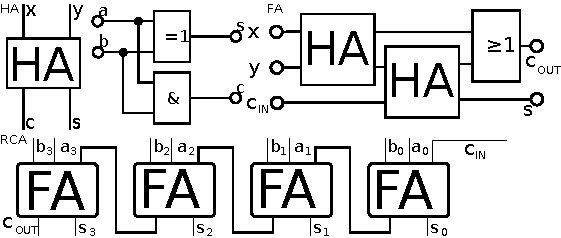
\includegraphics[width=0.5\textwidth]{Addierer}
\end{figure}
%\include{Halbaddierer.tex}
\textbf{Flip-Flops:} \emph{Arten:} RS-FF (Setzen-Rücksetzen), D-FF
(Data-Clock), T-FF (Toggle-Clock, lässt sich aus D-FF durch
Rückkopplung des negierten Ausgangs auf Eingang bauen), JK-FF (Jump-Kill-Toggle, immer
flankengesteuert oder als Master-Slave-FF),
\emph{Tabellen:}                                                                                             \\
\begin{tabular}{cc|c||c||c||cc|c}
$R$         & $S$      & $Q^+_{RS}$     & $Q_{D}$               & $Q^+_T$       & $J$ & $K$ & $Q^+_{JK}$     \\\hline
0           & 0        & bleibt         & $D$                   & $\bar{Q}_{T}$ & 0   & 0   & $Q_{JK}$       \\ 
0           & 1        & 1              &                       &               & 0   & 1   & 0              \\
1           & 0        & 0              &                       &               & 1   & 0   & 1              \\
1           & 1        & instabil       &                       &               & 1   & 1   & $\bar{Q}_{JK}$ \\
\end{tabular}                                                                                                \\
\emph{Schaltungen:}
\begin{figure}[H]
  \centering
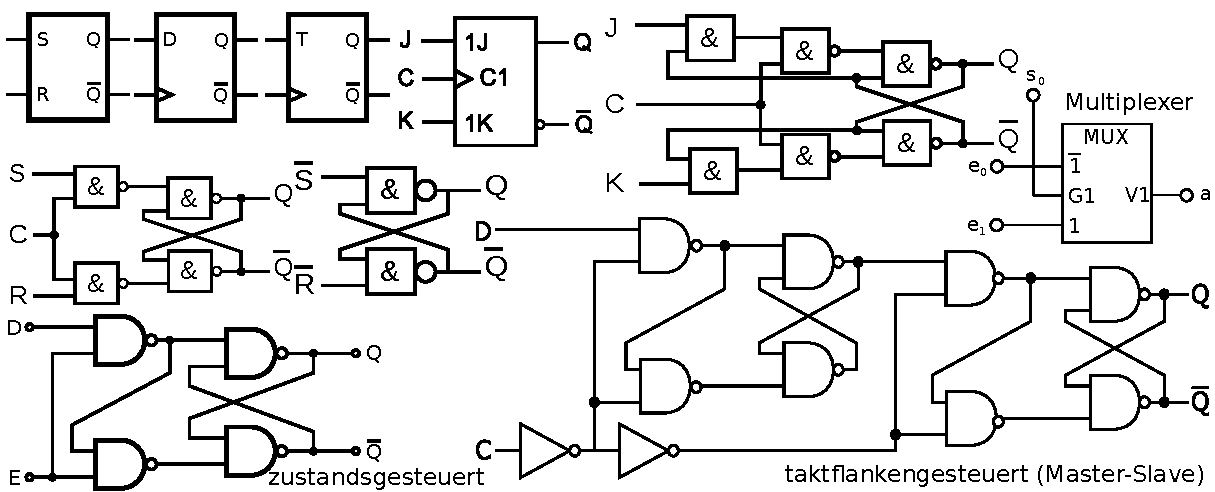
\includegraphics[width=0.5\textwidth]{Flipflops}
\end{figure}
\textbf{Multiplexer (MUX):} selektiert durchzulassenden Eingang auf
einen Ausgang, \textbf{Demultiplexer:} selektiert Ausgang auf den
einzelner Eingang ausgegeben werden soll (invers);

\paragraph{Zustandsautomaten:} \emph{Mealey-Automat:}
$\mathcal{A}=(Q,\Sigma,\omega,\delta,\lambda,q_0,F)$, ($Q$ Zustände (endlich)
mit $q_0$ Startzustand, $F$ Endzustände, $\Sigma$ endl. Alphabet,
$\delta:Q\times \Sigma\to Q$ Übergangsfunktion, $\lambda:Q\times
\Sigma \to \Omega$ Ausgabefunktion), \emph{Moore-Automat:} wie
Mealey-Automat, nur $\lambda:Q\to\Omega$.
\textbf{Sequentieller Automat:} Mit
Zuständen. \textbf{Kombinatorischer Automat:} Ohne Zustände.   

\paragraph{Cache.} \textbf{Lokalität:} \emph{Zeitl. \&
  räuml. Lokaliktät} (d.h. Daten, auf die gerade erst zugegriffen
wurde/ deren Adresse nahe bei solchen liegt, im Cache halten -
Wahrscheinlkt. für weitere Zugriffe hoch), Anwendung: räuml. Lok.:
ganze Blöcke geladen, zeitl. Lok.: Verdrängungsstrategien;
\textbf{Aufbau:} feste Anzahl von Cache-Einträgen, \emph{Cache-Eintrag:}
Adress-Tag $\rightarrow$ Cache-Line (Tag's werden gematcht,
Cache-Lines beinhalten Daten), \textbf{Adressaufteilung:} \fbox{Tag
  $\vline$ Index $\vline$ Wordadresse $\vline$ Byteadresse} (Länge
16/32/64 Bit je nach Adressraum/System); \textbf{Berechnung:}
$\#\text{Cache-Lines}=k\cdot\#\text{Indexbits} $ (für $k$-fach
assoziativen Cache),
$\text{Cache-Speicher}=\#\text{Cache-Lines}\cdot2^{\#\text{Wortbits}+\#\text{Bytebits}}$;
\textbf{Assoziativität $k$:} Anzahl der Sätze (direct-mapped (DM):
$k=1$, vollassoziativ (FA) $k=\#\text{Cache-Lines}$, kein Index),
\emph{Vor/Nachteile:} FA - viele (parallel arbeitende) Vergleicher
benötigt, weniger Verdrängung $\rightarrow$ hohe Effizienz \&
Hardwareaufwand, DM - weniger Vergleicher benötigt, mehr Verdrängung -
geringere Effizienz \& Hardwareaufwand; \textbf{Strategien:}
\textbf{Schreib-Hit:} \emph{write-back:} bei \texttt{WRITE} wird
Block zunächst im Cache abgelegt, Zurückschreiben in HS beim Ersetzen
der Cache-Line, \emph{dirty bit} wird beim Schreiben gesetzt - zeigt
an, ob HS + Cache übereinstimmen, \emph{write-through:} direktes
Zurückschreiben in HS, benötigt \emph{write buffer}, um Daten
zw. Cache \& HS zu Puffern; \textbf{Schreib-Miss:}
\emph{write-allocate:} zu schreibender Block wird in Cache geholt +
modifiziert (wird meist mit \emph{write-back} kombiniert),
\emph{non-write-allocate/write-around:} Block wird nicht in Cache geladen; 
\textbf{Verdrängungstrategien:} \emph{FIFO} (first in first out - zuerst in den Cache geladener Eintrag $\rightarrow$ zuerst ersetzt), \emph{LRU} (least recently used - am längsten ungenutzter Eintrag $\rightarrow$ zuerst ersetzt), \emph{LFU} (least frequently used - am wenigsten genutzer Eintrag $\rightarrow$ zuerst ersetzt, 1-2bits zu Speicherung der Häufigkeit), \emph{CLOCK/Round-Robbin}, \emph{optimal};
\textbf{MESI-Protokoll:} \emph{Ziel:} Gewährleistung von \emph{Datenkohärenz} bei MIMD-Systemen

\begin{figure}[H]
  \centering
  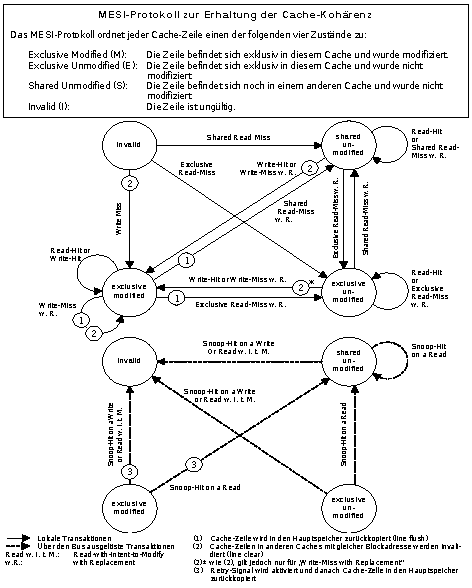
\includegraphics[width=0.5\textwidth]{MESI-Protokoll}
\end{figure}

\paragraph{Endianness.} \textbf{Big Endian:} MSB  (most significant bit zuerst), d.h. Wort ergibt sich direkt aus linearem Hintereinanderschreiben des Speicherinhaltes; \textbf{Little Endian:} Bytes des Wortes müssen invertiert werden; \textbf{Einordung verschiedener Architekturen:} 
\emph{Little Endian:} Intel x86-64 (I\emph{Intel convention}), 6502, Z80, MCS-48, DEC Alpha, Altera Nios II, PDP-11; \emph{Big Endian:} Motorola 6800 und 68k-Serie (\emph{Motorola convention}), IBM POWER, System/360-370 etc.

% RA II

\paragraph{Taxonomie von Rachnerarchitektur nach Giloi.} \emph{Tabelle:}
\begin{tabular}{p{0.25\textwidth}p{0.25\textwidth}}
Operationsprinzip & Hardwarestruktur \\
$\rightarrow$ Informationsstruktur\newline
$\rightarrow$ Steuerstruktur & 
$\rightarrow$ Hardwarebetriebsmittel\newline 
$\rightarrow$ Kooperationsregeln\newline 
$\rightarrow$ Verbindungstruktur \\
\end{tabular}
\emph{Weitere Unterteilung:} \textbf{Informationsstr.:} a) Klassen von
Datentypen (z.B.: Word, Feld, Stack, Liste etc.), b) Menge der
Maschinendarstellungen (z.B: IEEE754, 2er-Komplement), c) Menge von
Fkt.; \textbf{Steuerstr.:} a) Ablaufsteuerung (PC-getrieben
(Befehlszähler-getrieben),  datengetrieben, anforderungsgetrieben;
Datenzugriffssteuerung (Adresslogik, einfache Wertzuweisung,
assoziativer Zugriff)); \textbf{Hardwarebetriebsmittel:} a)
Prozessorstruktur (Verarbeitungseinheiten auf Core, Zusammensetzung
mehrerer Cores), b) Speicherstruktur (auch Register);
\textbf{Verbindungstruktur:} (z.B.: Bussysteme,
Single-/Multicore-System, Verbindungsnetzwerke); \textbf{Unterschied
  zu Brooks:} mehr Berücksichtigung der Interna (auf Nutzerseite);
\textbf{Beispieleinordnung:}
\emph{Steuerwerk}: RA $\rightarrow$ HWstr. $\rightarrow$
HWbetr.m. $\rightarrow$ Prozessorstruktur;
\emph{Register}: RA $\rightarrow$ HWstr. $\rightarrow$
HWbetr.m. $\rightarrow$ Speicherstruktur;
\emph{Speicherbus:} RA $\rightarrow$ HWstr. $\rightarrow$
Verbindungsstruktur;
\emph{Festkommaformat:} RA $\rightarrow$ Op.pr. $\rightarrow$
Inf.str. $\rightarrow$ Menge der Maschinendarst. \& Datenobjekte;
\emph{doppelt verkettete Liste:} RA $\rightarrow$ Op.pr. $\rightarrow$
Inf.str. $\rightarrow$ Klassen von Datenobj. $\rightarrow$
Strukturdatentypen;
\emph{Cache:} RA $\rightarrow$ HW.str $\rightarrow$ HW.b.m
$\rightarrow$ Speicherstruktur;
\emph{PC-getriebene Ablaufsteuerung:} RA $\rightarrow$ Op.pr. $\rightarrow$
Steuerstr. $\rightarrow$ Ablaufsteuerung;
\emph{Gleitkommaformat:} RA $\rightarrow$ Op.pr. $\rightarrow$
Inf.str. $\rightarrow$ Menge der Maschinendarst. \& Datenobjekte;
\emph{Assemblercode:} RA $\rightarrow$ Op.pr. $\rightarrow$
Inf.str. $\rightarrow$ Menge von Fkt.;
\emph{Verbindungsnetzwerk:} RA $\rightarrow$ HW.str. $\rightarrow$
Verbindungsstr.;

\paragraph{Brooks Definition (60/70er Jahre).} interne Struktur \&
Organisation des Rechners vor Nutzer verborgen, RA$=$
Interfacebeschreibung/Programmierschnittstelle (Befehlssatz, Speicherstruktur,
Adressierungsmodi, Registerstuktur, Unterbrechungsbehandlung,
E/A-Fkt. etc.) 

\paragraph{Moore's Law.} Verdopplung der Transistoren auf Chips pro 10
Monate (Erhöhung der Prozessorleistung, Einergieaufnahme $\sim f^2$
$\rightarrow$ Taktfrequenz seit 2006 nicht mehr gesteigert, Lücke
zwischen Speicher- \& CPU-Performance wächst);

\paragraph{Flynnsche Klassifikation.} \textbf{SISD:}
Von-Neumann- \& Harvard-Architektur, Single-Core-PC; \textbf{SIMD:}
Vektor- \& Feldrechner; \textbf{MISD:} leere Klasse; \textbf{MIMD:}
Multicoresysteme;
(S\ldots \emph{single}, M\ldots \emph{multiple}, I\ldots
\emph{instruction}, D\ldots \emph{data});
\begin{figure}[H]
  \centering
  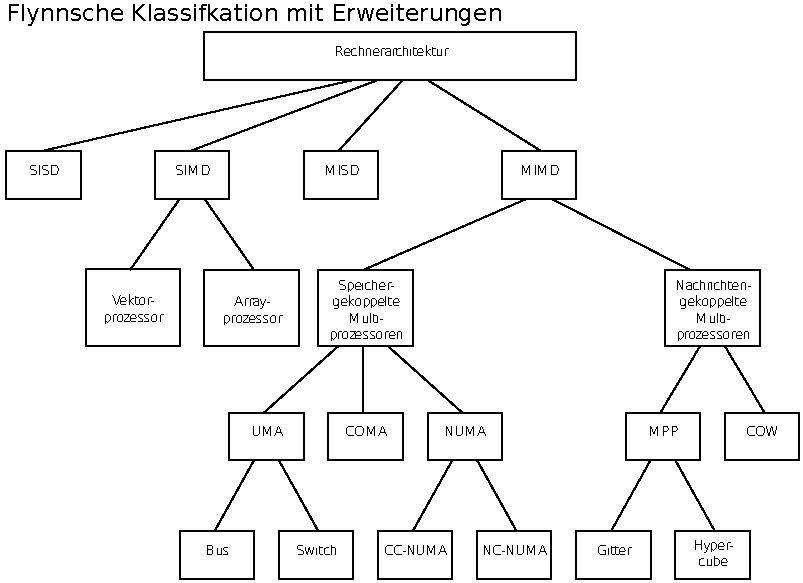
\includegraphics[width=0.5\textwidth]{FlynnscheKlassifikation}
\end{figure}

\paragraph{Speichergekoppelte Multiprozessoren.} \textbf{Symmetrische Multiprozessoren (SMP).} Gleichartige Prozessoren über Bus/Kreuzschinenschalter/mehrstufiges Netzwerk verbunden; 
\textbf{Distributed-shared-memory-Systeme (DSM):} einheitl. Adressraum, aber Speicher physikalisch auf einzelne Verarbeitungsknoten verteilt; \textbf{UMA-Multiprozessoren (uniform memory acces):} alle Prozessoren greifen gleichermaßen af gemeinsamen Speicher zu (gleiche Zugriffszeit); jeder Prozessor kann lokalen Cache besitzen, Nutzen des Snooping-Bus-Verfahrens (Cache-kohärent), auch SMP genannt; \emph{Beispiele:} Sun Enterprise 10000, \textbf{NUMA (non-uniform memery access):} Zugriffszeiten auf gemeinsamen Speicher variieren nach Ort der Speicherzelle (durch Verbindungsnetzwerk induziert); Speichermodule physikalisch auf Verarbeitungsknoten verteilt; gemeinsamer Adressraum; prozessorlokale Caches; \emph{Beispiele:} Connection Machine CM-5 von TMC,  \textbf{CC-NUMA (cache coherent NUMA):} Caches über gesamtes NUMA-Systems kohärent organisiert (directory-based coherence protocol); Datenbank über Befinden der einzelnen Cache-Zeilen \& Zustand; \emph{Beispiele:} Sequent NUMA-Q (4 Pentium Prozessoren mit L1-/L2-Cache, bis zu 4GB RAM), AMD-Mehrprozessorsysteme auf OPTERON-Basis, SGI-Systeme mit NUMAlink, früher: basierend auf Alpha-Prozessor EV7 (Digital Equipment Corporation), MIPS-R1x000-Prozessoren (SGI-Origin-Serie); \textbf{NCC-NUMA (non-cache-coherent NUMA):} NUMA ohne Cache-Kohärenz; lokale Speicherzugriffe (über Caches) und entfernte Zugriffe (vorbei an Caches); \emph{Beispiele:} CRAY T3E (Vektorrechner); \textbf{COMA (cache-only mememory architecture):} Spezialfall des CC-NUMA; physikalsch verteilte Speichermodule ausschließlich Caches; gemeinsamer Adressraum; Speicher zieht benötigten Speicherblöcke an (\emph{attraction memery} Prinzip); \emph{Beispiele:} KSR 1, KSR 2 (Kandall Square Research);

\paragraph{MMX, SSE, AVX.} \textbf{MMX (multi media extension - 1996):} große Register (64bit) werden
in kleinere Register aufgeteilt, die parallel mit
einem Befehl verarbeitet werden können (\emph{PackedByte} ($8\times 8$bit),
\emph{PackedWord} ($4\times 16$bit) , \emph{PackedDoubleWord}
($2\times32$bit), \emph{QuadWord} ($1\times 64$bit)); SIMD (Feldrechnerprinzip);
Erweiterung für IA-32-Prozessorarchitektur; für Integer-Datenpakete \textbf{SSE (streaming
  SIMD extension - 1999):} große Register (128bit) in
z.B. $4\times32$bit Register aufgeteilt (parallel verarbeitend); SIMD
(Feldrechnerprinzip); Befehlssatzerweiterung für
\texttt{x86}-Prozessorarch., speziell für Floating-Point-Datentypen;
8-16 Register, die mit \texttt{xmmi} (\texttt{i} variabel) beschriftet sind)
\textbf{AVX (advanced vector extensions - 2008):} Vergrößerung der
SIMD Register auf 256bit; neues 2-Operandenformat $a:=b+c$, dadurch
wird Quellregister nicht zerstört (SSE-Befehle $a:=a+b$ im Zweioperandenformat); Sandy-Bridge realisiert als erstes AVX2;

\paragraph{Speicherhierarchie (Bsp.daten).} 1. \textbf{Register} (512, direkt),
2. textbf{Caches} L1 (32 kByte, 3 Takte), L2 (256 kByte, 8 Takte), L3 (8
MByte, 15 Takte), 3. \textbf{RAM/Hauptspeicher} (4/8 GByte, 100/120 Takte), 4. \textbf{Festplatte}
(1TByte, Mio. Takte);

\paragraph{Adressierung.} \textbf{Aufbau Befehlswort:}\\
\fbox{Operationscode $\vline$ Operanden $\vline$ Adressteil}\\
\textbf{Adressierungsarten.} \textbf{Immediate Operand:}
Direkt-Operanden-Adressierung (d.h. ein Register wird für Operanden
nicht gebraucht), Operand als Konstante im Befehl (z.B.: Assembler (\#)
\texttt{ADD R1,\#17} oder \texttt{MOVE.B R3, \#225}); \texttt{Immediate
  Adress:} effektive Adresse steht als absolute Adresse im Befehl,
Operand im Speicher;
\textbf{Register Direct:} Adresse steht als kurze Registeradresse im
Befehl, Operand steht im Register (z.B.: \texttt{MOVE.W SP,R0} -
transportiert Inhalt von \texttt{R0} in Stackpointerregister);
\textbf{Register Indirect:} effektive Adresse steht im Register,
Operand im Speicher (z.B.: Assembler (\texttt()) \texttt{MOVE.H
  R1,(R0)} - transportiert 16bit-Operanden, dessen Adresse in
\texttt{R0} liegt nach \text{R1}); \textbf{Register Indirect \&
  Displacement:} im Register stehende Adresse wirkt als Basisadresse,
Offset/Displacement steht im Befehl und muss zu ihr addiert werden;
Operand im Speicher
(z.B.: \texttt{MOVE.H R2 \#4(R3)}) \textbf{Scaled Index
  Addressierung:} wie Register Indirect mit Displacement nur dass
zusätzlich noch $\text{scale}*\text{index}$ zur Adresse addiert wird;
\emph{scale} muss 2er Potenz sein (dann wird Multiplikation, die nicht
möglich ist, zu Bitshifting); \textbf{Implizite Adressierung:} es wird
implizit ein Register für den Opcode verwendet (z.B.: \texttt{ADD R5}
bei Addition mit Akkumulator und Rückschreiben auf diesen, oder
\texttt{ADD R3 R4} (2-Operandenformat, bei dem auf ersten
Op. geschrieben wird); \textbf{Überdeckte Adressierung:} Ergebnis
stimmt mit einem Operanden überein (z.B.: \texttt{ADD R1 R2});
\textbf{$n$-Adress-Format:} typische Operandenanzahl bei \texttt{ADD},
\texttt{SUB}, \texttt{AND} und \texttt{OR}; (z.B.: bei
0-Adress-Maschine - beide Operanden auf Stack in ALU, 1-Adress-Format
- ACCU als impliziter, überdeckter Operand; 2-3 Adressformat - GPR (general purpose register)); 

\paragraph{Von-Neumann-Architektur.} \textbf{Komponenten:} CPU,
Systembus, Hauptspeicher, E/A-Einheit; \emph{CPU:} beinhaltet
CU/Steuerwerk (Befehlszähler, Befehlsregister, Befehlsdekoder, Steuer-
\& Statusregister/Stackmodul, zentrale Steuerschleife), Rechenwerk
(ALU, Akkumulator - log./arithm. Op., Interaktion mit Steuerwerk durch
arithm. Flags); \emph{HS:} Daten \& Befehle, gebildet durch linear
adressierte Von-Neumann-Variablen (IS+value), zugriff auf gemeinsamen
Bus; \emph{Bus:} Adress-, Daten-, Steuerbus, für Befehle \& Daten,
Einschr. der Parallelität; \textbf{Befehlsabarbeitung (Von-Neumann-Zyklus):}
0. Befehlsadresse im Befehlszähler, 1. IF (instruction fetch), 2. ID
(instruction decode)(3. OF (operand fetch)) 3. EX (execute), 4. WB
(write back);
\emph{Schemata:}
\begin{figure}[H]
  \centering
  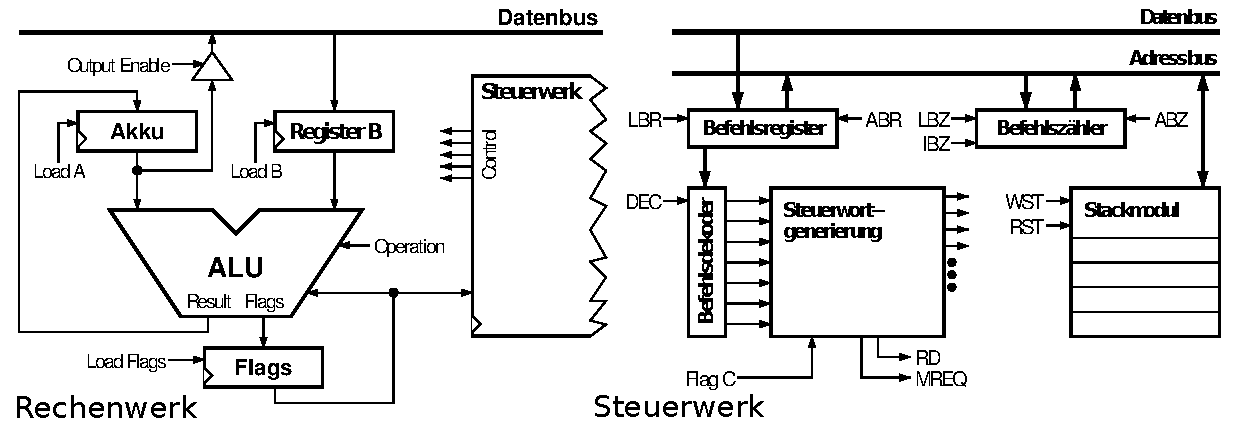
\includegraphics[width=0.5\textwidth]{Rechen&Steuerwerk}
\end{figure}
\textbf{Nachteile:} Daten \& Befehle haben gemeinsamen Bus/Speicher;
sequentielles Arbeiten (ein Kontrollfluss/ Von-Neumann-Zyklus (In-Order-Execution));
CPU-Speicher-Geschwindingkeitsunterschied; \textbf{Lösung:}
Paralellisierung (Pipelining, Multicore, Multithreading, superskalare Befehlsabarbeitung), out-of-order-execution,
Caching, getrennter L1-Cache für Befehle und Daten; 

\paragraph{Beispiel: Arbeitsweise Steuerwerk.} \textbf{Generelle Abarbeitung von Befehlen (hier z.B.: \texttt{JC} mit Bedingungsflag $C$):} 1. Befehlswort anfordern, (d.h. Befehlszähler auf Adressbus legen \texttt{ABZ}, HS anfordern \texttt{MREQ}, HS lesen \texttt{RD}), 2. Wartetakt \& Befehlszähler inkrementieren \texttt{IBZ}, 3. Befehlswort vom Speicher (Datebus) in Register laden (\texttt{LBR}), 4. wenn $C$, Adressteil des Befehlsregisters auf Adressbus (\texttt{ABR}), Befehlszähler vom Adressbus laden (\texttt{LBZ}); (4. Schritt bei \texttt{CALL} wäre z.B.: Befehlszähler auf Adressbus ausgeben (\texttt{ABZ}) und auf Stack legen (Rücksprungadresse) (\texttt{WST}), Adressteil des Befehlsregisters auf Adressbus ausgeben \texttt{ABR}) und in BZ laden (\texttt{LBR});

\paragraph{Harvardarchitektur.} \textbf{Unterschied zu VN-Arch.:}
Befehle \& Daten in unterschiedl. Speichern \& benutzen
unterschiedl. Busse; \textbf{Anwendung:} L1-Caches,
Pipeline-Prozessoren; \textbf{Vorteil:} Parallelität beim Laden von
Befehl+Operand, kein Gegenseitiges Verdrängen (Cache)/Überschreiben möglich;


\paragraph{RISC/CISC:} \textbf{RISC:} wenig Befehlsformate fester
Länge, \texttt{LOAD}/\texttt{STORE}-Architektur,
viele Register (bis zu 256), direkte Verdrahtung der Befehle im
Dekoder (kein Mikrocode $\rightarrow$ schnellere Ausführung),
\emph{Vorteile:} schnelleres Dekodieren; weniger Hardwareaufwand;
Sparsamkeit bei Adressierung, wenn $R0$ fest auf $0$ verdrahtet;

\paragraph{Verbindungsnetzwerke.} \textbf{statisch:} jeder Knoten hat
feste Leitungen zu Nachbarknoten (Links), Netzwerk beschränkt sich auf
Verbindungsleitungen, Verbindungs- \& Vermittlungsfunktion nicht
Bestandteil; \textbf{dynamisch:} Verbindungen schaltbar, konkrete
Verbingung erst zu Kommunikationszeitpkt. vorhanden;
\textbf{Kenngrößen:} \emph{Grad} $d(v)$, \emph{Durchmesser} $d$, \emph{mittl. Abstand} $\bar{d}$, \emph{Halbierungsbreite} $b$ (minimal zu läschende Kantenanzahl, damit Netzwerk in 2 gleichgroße Teile zerfällt), \emph{kleinste Erweiterung} $e$, \emph{Einbettung} (i. gaphentheoretischen Sinn), \emph{Konnektivität} $k:=\min\{k_V,k_E\}$, \emph{Knotenvernetzung} $k_V$ (minimal zu löschende Knotenzahl, damit Netzwerk in 2 Teile zerfällt), \emph{Kantenkonnektivität} $k_E$ (analog für Kanten);
\textbf{Entwurfsziele:} kleiner, konst, Grad, einfach skalierbar, kleiner Durchmesser, hohe Konnektivität, viele unabh. Pfade zw. 2 Knoten, hohe Halbierungsbreite; \textbf{Speziell für High Performance Computing (HPC)/Cluster Computing:} wenige Schaltzellen, gutes Blockierungsverhalten, geringe Latenz, hohe Übertragungsrate;\\
\begin{tabular}{c|ccccc}
                     & $d(v)$        & $d$                      & $k$         & $b$               & $e$   \\ \hline
Ring $C_n$           & 2             & $\floor{n/2}$            & 2           & 2                 & 1     \\
Graph $K_n$          & $n-1$         & 1                        & $n-1$       & $\floor{n^2/4}$   & 1     \\
Stern $S_n$          & 1,$n-1$       & 2                        & 2           & $\floor{n/2}$     & 1     \\
Binärb. $B_n$        & 1,2,3         & $2\log_2(\frac{n+1}{2})$ & 1           & 1                 & $n+1$ \\
2D Torus $T_n$       & 4             & $2\floor{n/2}$           & 4           & $2(\sqrt{n}+[1])$ & 
$2\sqrt{n}+1$                                                                                             \\
H.-cube $H_n$        & $\log_2{n}$   & $\log_2{n}$              & $\log_2{n}$ & $n/2$             & 
$n$                                                                                                       \\
$r$D Gitt. $G_{r,n}$ & $r,\ldots,2r$ & $r(\sqrt[r]{n}-1)$       & $r$         & -                 & -     \\
\end{tabular}
\textbf{Bsp.: $n\times n$-Omega-Netzwerk:} \textbf{Aufbau:} $2\times
2$-Crossschalter (Betazellen) in $\log_2{n}$ Stufen angeordnet, jede
Stufe enthält $n/2$ Schalter, 'perfect shuffeling';
\textbf{Destination Routing:} Quell- \& Zieladresse implizieren
Schalterstellung (\emph{destination tag}) durch \textbf{XOR-Routing:}
$\text{Quelladresse}\dirplus\text{Zeiladresse}=c_{\log_2{n}-1}\ldots c_0$ ergibt die nötigen
Schalterstellungen (Schalter $i$-ter Stufe: $c_i=0$ ungekreuzt
('straight'), $c=1$ vertauschen ('exchange')); \textbf{Kollision:}
tritt auf, wenn $\text{Quelle}_1\text{Ziel}_1$ mit
$\text{Quelle}_2\text{Ziel}_2$ in mindestens $\log_2{n}$ bits
übereinstimmen; 

\begin{figure}[H]
\centering
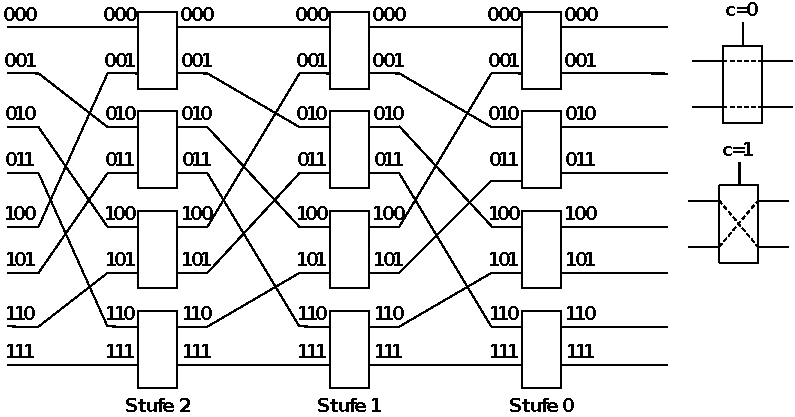
\includegraphics[width=0.5\textwidth]{Omega-Netzwerk}
\end{figure}
\begin{figure}[H]
\centering
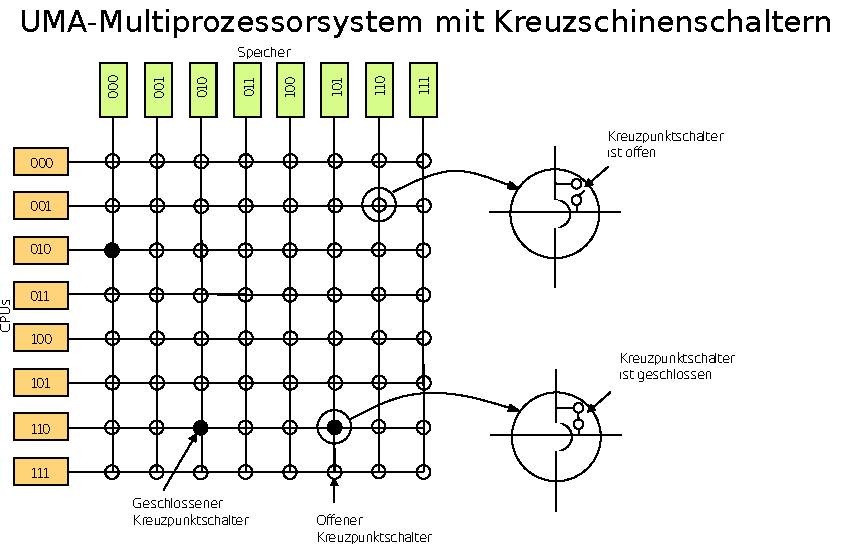
\includegraphics[width=0.5\textwidth]{Kreuzschinenverteiler}
\end{figure}

\paragraph{Paketvermittlung.} Nachricht in Pakete aufgeteilt; Pakete
werden unabh. voneinander durch Netzwerk transportiert;
\textbf{Paket:} besteht aus \emph{Header} (Routing- \&
Kontrollinformation), \emph{Datenteil} (Anteil der Gesamtnachricht),
\emph{Endstück} (\emph{trailer}, enthält Fehlerkontrollcode);
\textbf{Arten:} \textbf{Store-and-Forward:} gesamtes Paket in jedem
Zwischenknoten komplett gespeichert vor Weiterleitung; \emph{Vorteil:}
schnelle Freigabe von Verbindungen; \emph{Nachteil:} schlechte Latenzzeiten,
große Puffer je Knoten; \textbf{Virtual-Cut-Through:} Pakete in
\emph{phits} (physical units) unterteil, pipeline-artig durch Netz
transportiert; an jedem Zwischenknoten wird nur Header betrachtet; bei
freier Verbingung $\rightarrow$ Weiterleitung; bei Blockierung
$\rightarrow$ Sammeln im letzten Erreichbaren Knoten; Vorteil:
Freigabe des bisherigen Weges durch Puffern des Pakets im
Knotenpuffer; Nachteil: große Puffer (entartet bei Block. zu
Store-and-Forward); \textbf{Wormhole-Switching:} wie
Virtual-Cut-Through, aber bei Blockierung bleiben alle phits an iherer
Position; \emph{Vorteil:} kleine Puffer, bessere Latenzzeiten;
\emph{Nachteil:} bisheriger Weg wird evtl. blockiert; \textbf{Leitungsvermittlung:}
Leitung wird stationar aufgebaut und bleibt für gesamte
Übertragungsdauer; \emph{Nachteil:} Knoten werden blockiert, obwohl schon
alle phits passiert haben, ineffizient für HPC (\emph{high performance
  computing}); \emph{Vorteil:} hohe Nettoübertragungsrate (keine
Zeilcodierungen mitgeführt), hohe Leitungsstabilität;

\paragraph{Parallelisierung:} \textbf{Kennwerte (nach RA I):} $CPI$ - Taktzyklen
pro Befehl; $IPC$ - Instruktionen pro Zyklus; $t$ Arbeitszeit; $T$
Periodendauer Takt; $f$ Taktfrequenz; \textbf{Berechnung (nach RA I):} 
\begin{tabular}{|ll|}
\hline
\textbf{Laufzeit}            & $t=\#\text{Befehle}\cdot CPI\cdot T=\frac{\#\text{Befehle}\cdot T}{IPC}$ \\
\hline
\end{tabular}                                                                                           \\
\textbf{Vergleich: sequentieller vs. hypothetischer Parallelrechner.} Gegeben: bestimmte Berechnungsvorschrift, testen auf Parallelisierbarkeit; \textbf{Kennwerte (RA II):} \emph{Größen:} $Z_p$ (Anzahl der Instruktionen bei Algo. mit $p$ Prozessoren, $Z_1$ heißt seriell), $T_p$ (Laufzeit bei $p$ Prozessoren in Takten)
\begin{tabular}{|ll|}
\hline
\textbf{Speed-Up}            & $S_p=T_1/T_p$                                                            \\
\textbf{Effizienz}           & $E_p=S_p/p$                                                              \\
\textbf{Operationsredundanz} & $R_p=Z_p/Z_1$                                                            \\
\textbf{Auslastung}          & $U_p=\frac{Z_p}{pT_p}$                                                   \\
\textbf{Effektivität}        & $F_p=\frac{S_pE_p}{T_1}$                                                 \\
\hline
\end{tabular}\\
\textbf{Beispiel:}
\begin{figure}[H]
  \centering
  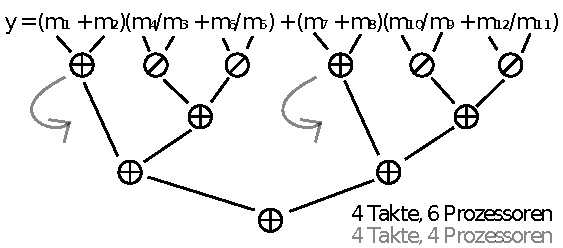
\includegraphics[width=0.2\textwidth]{Parallelisierungsbeispiel}
\end{figure}

\paragraph{Pipelining.} \textbf{Beschreibung:}  gestaffelt paralleles
Abarbeiten von Befehlen (IF-, ID-, EX-, WB-Stufen von Befehlen
gestaffelt nebeneinander laufen lassen); \textbf{Berechnung der Effizienzsteigerung (nach RA I):}                                      \\
\begin{tabular}{|ll|}
\hline
\textbf{Laufzeit (seriell)}  & $t_{\text{Pipeline}}=(\#\text{Pipeline-Stufen}+\#\text{Befehle}-1)\cdot T_{\text{Takt}}$ \\
\textbf{Laufzeit (Pipeline)} & $t_{\text{seriell}}=\#\text{Pipeline-Stufen}\cdot\#\text{Befehle}\cdot T_{\text{Takt}}$; \\
\textbf{Speed-Up}            & $SP=t_{\text{seriell}}/t_{\text{Pipeline}}$                                              \\
\textbf{Effizienz}           & $EF=SP/S=\frac{\#\text{Befehle}}{\#\text{Befehle}+\#\text{Pipelinestufen}-1}$            \\
\hline
\textbf{Asympt. Werte}       & $EF\upto 1$, $SP\upto S$, $CPI\downto 1$ (für $\#\text{Befehle}\to\infty$)               \\
\textbf{Effektive Werte}     & $SP<\#\text{Pipelinestufen}$, $EF<1$, $CPI>1$                                            \\
\hline
\end{tabular}

\paragraph{Out-of-Order-Execution.} bei superskaleren Prozessoren (d.h. mehrere Funktionseinheiten wie ALU, FPU, Lade-\&-Speichereinheit, Vektoreinheiten,; hohe Befehlsparallelität ($IPC>1$ - \underline{$IPC$-fach superskalar})); \textbf{Arbeitsweise:} 1. IF (instruction fetch - Befehl laden), 2. IB (instruction buffer - Befehl in Warteschlange), 3. Warten des Befehls im Buffer auf Operanden (dann Verslassen des Buffers), 4. Befehl an passende Fkt.einheit Übergeben \$ ausgeführt, 5. Ergebnis in Ergebniswarteschlange eingetragen (\emph{register retirement/buffer}), 6. Nach Schreiben aller Ergebnisse früherereingetroffener, im Programmcode älterer Befehle $\rightarrow$ Schreiben des Resultats in Register; \textbf{Beispiel:} $f=2,8\text{GHz}$, $3$-fach superskalar ($IPC=3$), $70\text{ns}$ Speicherlatenz ($\rightarrow$ $2,8\cdot 70=196$ Takte): In der Zeit werden $3\cdot 196=588$ Befehle abgearbeitet (d.h. potentiell 588 Bufferplätze $\rightarrow$ 128 wäre noch realistisch, da festverdrahtet, großer HWaufwand, Datenabhängigkeiten etc.); 

\paragraph{Pipeline-/Out-of-Order-Execution-Konflikte (Hazards):} \textbf{Datenhazard:} \emph{read
  after write (RAW):} z.B.: \texttt{\underline{R1} = R2 + R3; R4 = \underline{R1}+\#1}, da
erster Operand in 2. Anweisung eventuell noch nicht gestored wurde,
müsste 2. Anweisung warten; 'Shortcuts' im Datenweg der Pipeline
helfen; \emph{write after read (WAR):} z.B.: \texttt{R1 = \underline{R2}+R3; \underline{R2} =
  \#2;}, Schreiben könnte vor Lesen stattfinden; tritt bei Pipeline
eher nicht auf; \emph{write after write (WAW):} z.B.:
\texttt{\underline{R1} = R2+R3; \underline{R1} = \#2}, falsche
Schreibreihenfolge führt zu falschem Ergebnis; \textbf{Steuer/Kontrollhazards:}
treten bei Instruktionen auf, die Befehlszähler verändern (z.B.: \texttt{JMC}), \emph{Lösungen:} Sprungvorhersage
(zusätzliche Hardwareeineheit, die Sprungwahrscheinl. berechnet);
Delayed Branching (in der Zeit, in der Sprungziel ermittelt wird,
werden andere unabh. Berechnungen durchgeführt),
\textbf{Strukturhanzards:} mehrere Pipelinestufen griefen auf gleiche
Ressource (z.B.: Quellregister) zu; \emph{Lösungen:} Shortcuts
innerhalb der Pipeline/ Anhalten der Pipeline (NOP);

\paragraph{Leistungsbewertung.} \textbf{Kenngrößen:} \textbf{IPS:}
instructions per second; \textbf{IOPS:} integer operations per second;
\textbf{FLOPS:} floating point operations per second; \textbf{IOOPS:}
I/O operations per second (\texttt{READ, WRITE, RANDOM} etc.), nur \underline{ein Kern} \& \underline{keine Spezialregister} benutzt; 
\textbf{Theoretische Peak-Performance:} theoretische maximal
Erreichbarer Durchsatz eines Systems mit mehreren Kernen \& Spezialregistern (z.B.: FPPP - floating point peak performance);
\textbf{Beispielrechnung:} $f=330\text{MHz}$, $IPC=4$ (superskalar/Pipeline), $IOPC=2$, $FLOPC=2$; Dann: $IPS=IPC\cdot f=1,32\text{GIPS}$, $IOPS=f\cdot IOPC=660\text{MIOPS}$, maximale $IOOPS=f\cdot IOOPC=330\text{MHz}\cdot 16=5,28\text{GIOOPS}$ (Faktor 16: $4\times 1$ IF, $4\times 1$ WB, $4\times 2$ OF bei 2/3-Adressbefehl); Bei Akkumulator hier z.B. nur Faktor 2 (IF und OF, Akku kostet nichts);


\paragraph{Vektorrechner.} \textbf{Funktionsprinzipien:} \emph{SIMD} (bei nur
einem Vektorprozessor), viele  \emph{Speicherbänke} kein Cache,
\emph{Skalareinheit} für nicht vektorisierbare Probleme, mehrere
Vektoreinheiten pro Vektorprozessor; meist mehrere Vektorprozessoren (damit als Ganzes
MIMD), \emph{arithmetisches Pipelining} (einzelne Phasen eines Befehls in
einer Pipeline-Form organisiert, z.B.: FP-Add: 1. Exponenten
vergleichen, Differenz, 2. Rechtsshift der Mantisse des kleineren
Operanden, 3. Festkommaaddition der Mantissen, 4. Normalisierung),
\emph{Chaining} (Hintereinanderschalten von Pipelines, z.B.: bei
$A=B.*C + D$ (elementweise Mult.) erste Addition, dann
Multiplikation), nach Möglichkeit paralleler Zugriff auf HS;

\paragraph{Feldrechner.} \textbf{Aufbau:} besteht aus $N$
gleichartigen Einheiten (\emph{processing elements} (PE)), die durch
Verbindungsnetzwerk Daten austauschen können und eine gemeinsame
Steuerung (\emph{control unit} (CU)) haben);
\textbf{Verarbeitungsprinzip:} \emph{Pipelining}, \emph{Chaining};
\textbf{Anwendung:} MMX, SSE, AVX;

\paragraph{Vergleich: Vektorrechner/Cache-basierend.}
\textbf{Vektorrechner.} maximale Performance für große Probleme; Einbruch, wenn Vektorregister voll ist \& für
einen einzelnen Wert ein fast leeres Register genutzt werden muss
(wegen Laden des neuen Registers; $k$-faches der Registerlänge); bei
$n\times n$-Matrix quadratisches Wachstum der Problemgröße in $n$
$\rightarrow$ rascher Leistungsanstieg; \textbf{Cache-Rechner.}
maximale Leistung for kleine Probleme für die L1-Cache reicht;
Einbrüche immer beim Erreichen der nächst höheren Speicherhierarchie
(L2/L3-Caches \& Auslagerung auf RAM (\emph{paging}));
\emph{Beispiel Matrix-Multiplikation Floating-Point-Leistungskurven.}
\begin{figure}[H]
  \centering
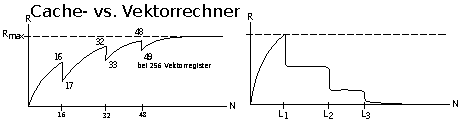
\includegraphics[width=0.5\textwidth]{Cache-Vektorrechner}
\end{figure}

\paragraph{Systolisches Array.} \textbf{Definition:} zellulärer Automat, der aus
gleichartigen, im Raum gleichmäßig angeordneten und gekoppelten Zellen
besteht; Kopplungsmuster ist lokal; es tritt kein Broadcasting \&
Rippling auf; \textbf{Rippling:} Hindurchplätschern von Daten durch
Zellen; \textbf{kein Rippling:} System getaktet; Freigabe des Signals
zum Taktzeitpunkt; \textbf{Analogie zum Feldrechner:} siehe
Feldrechner (PEs); \textbf{Analogie zum Vektorrechner:}
Verallgemeinerung des Pipeline-Prinzips (1D - einfache Pipeline, 2D -
Pipelines die sich in regulärer Weise beeinflussen);
\textbf{Bedeutung:} Spezialrechner für Signal- und Bildverarbeitung;
\begin{figure}[H]
  \centering
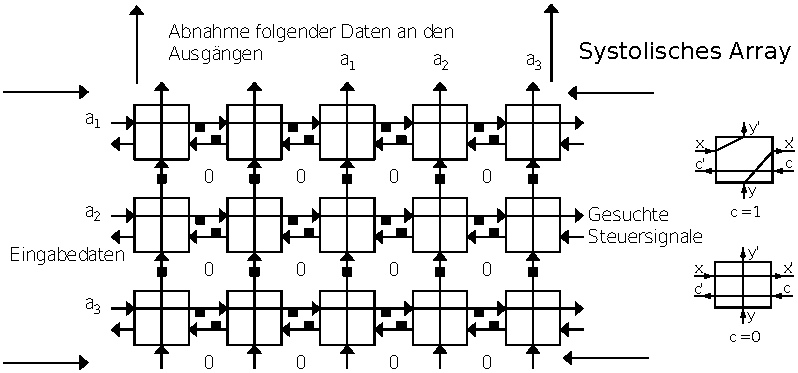
\includegraphics[width=0.5\textwidth]{SystolichesArray}
\end{figure}

\paragraph{ECS:} $t_{\text{Rechnertyp}}=(k[*k'],d[*d'],w[*w'])$; $k$\ldots Anzahl der nebenläufigen Steuerwerke, $k'$\ldots Anzahl der spezialisierten Steuerwerke für Programm/Prozessorpipelining; $d$\ldots Anzahl der nebenläufigen Rechenwerke (je Steuerwerk), $d'$\ldots Anzahl der Pipelining Rechenwerke (je Steuerwerk), $w$\ldots Anzahl der parallelen Bitstellen im Rechenwerk (z.B.: AVX: 256bit/ SSE 128/ MMX 64bit) ($W'$\ldots Anzahl der elementaren Teilwerke);

\paragraph{HDN (hardware description notation) \& DLX.} \textbf{DLX:}
hypothetische Prozessorarchitektur mit RISC-Befehlssatz \& 32 \underline{32bit}-Registern (GPR) (Vorbild MIPS); Speicher ist \underline{byteadressiert} \\
\begin{tabular}{ll}
\texttt{R0} null; unveränderlich & \texttt{R1} reserviert für den Assembler                \\
\texttt{R2-R3} Funktionsrückgabewerte & \texttt{R4-R7} Funktionsparameter                  \\ 
\texttt{R8-R15} beliebig              & \texttt{R16-R23} Registervariablen                 \\ 
\texttt{R24-R25} beliebig             & \texttt{R26-R27} reserviert für das Betriebssystem \\ 
\texttt{R28} Globaler Pointer         & \texttt{R29} Stackpointer                          \\ 
\texttt{R30} Registervariable         & \texttt{R31} Rücksprungadresse                     \\
\end{tabular}
\textbf{Befehlsformate:} \emph{Register-Befehlsformat (R)}, \emph{Immediate-Befehlsformat (I)}, \emph{Jump-Befehlsformat (J)}:\\
\begin{tabular}{| l | c | c | c | c | c | c |}
\hline
  & 109876 & 54321 & 09876 & 54321 & 09876  & 543210                  \\\hline
R & 000000 & Rs1   & Rs2   & Rd    & unused & opcode                  \\\hline
I & opcode & Rs1   & Rd    & \multicolumn{3}{|c|}{immediate ($\imm$)} \\\hline
J & opcode & \multicolumn{5}{|c|}{value ($\val$)}                     \\\hline
\end{tabular}

\emph{Tabelle:}                                                                                          \\
\begin{tabular}{llcl}
\textbf{Instr.} & \textbf{Description} &     & \textbf{Operation}                                        \\
ADD(I)(U)       & add	(i) (u)        & R/I & $Rd \leftarrow Rs_1 + \iu$                                \\	
AND(I)          & and (i)    	       & R/I & $Rd \leftarrow Rs_1 \& \imme$                             \\
BEQZ            & branch if $=0$       & I   & $PC \leftarrow PC + ext(\imm)$ if $Rs_1 = 0$              \\
BNEZ            & branch if $\neq 0$   & I   & $PC \leftarrow PC + ext(\imm)$ if $Rs_1 \neq 0$           \\
J               & jump                 & J   & $PC \leftarrow PC + ext(\val)$                            \\
JAL             & jump and link        & J   & $R_{31} \leftarrow PC + 4 ; PC \leftarrow PC + ext(\val)$ \\
JALR            & jump and link reg.   & I   & $R_{31} \leftarrow PC + 4 ; PC \leftarrow Rs_1$           \\
JR              & jump register        & I   & $PC \leftarrow Rs_1$                                      \\	
LHI             & load high bits       & I   & $Rd \leftarrow \imm <<16$                                 \\
LW              & load word            & I   & $Rd\leftarrow_{32}\mem[Rs_1 + ext(\imm)]_{0..31}$         \\
OR(I)           & or                   & R/I & $Rd \leftarrow Rs_1 | \imme$                              \\
SEQ(I)          & set if $=$ to (i)    & R/I & $Rd \leftarrow (Rs_1 = ext(\imme) ? 1 : 0)$               \\
SLE(I)          & set if $\leq$ (i)    & R/I & $Rd \leftarrow (Rs_1 \leq ext(\imme) ? 1 : 0)$            \\
SLL(I)          & shift l. logic. (i)  & R/I & $Rd \leftarrow Rs_1 \ls (\imme\% 8)$                      \\
SLT(I)          & set if $<$ than (i)  & R/I & $Rd \leftarrow (Rs_1 < ext(\imme) ? 1 : 0)$               \\
SNE(I)          & set if $\neq$ to (i) & R/I & $Rd \leftarrow (Rs_1 \neq ext(\imme) ? 1 : 0)$            \\
SRA(I)          & shift r. arithm. (i) & R/I & $Rd \leftarrow Rs_1 \rsa (\imme\% 8)$                     \\
SRL(I)          & shift r. logic. (i)  & R/I & $Rd \leftarrow Rs_1 \rs (\imme\% 8)$                      \\
SUB(I)(U)       & subtract (i) (u)     & R/I & $Rd \leftarrow Rs_1 - Rs_2$                               \\
SW              & store word           & I   & $\mem[Rs_1 + ext(\imm)]_{0..31} \leftarrow_{32}Rd$        \\
XOR(I)          & exclusive or (i)     & R/I & $Rd \leftarrow Rs_1 \hat{\:} \imme$                       \\
\end{tabular}

\begin{tabular}{ll}
Transfer        & $\leftarrow$   \\
Speicher        & $\mem$         \\
Trans. Länge    & $\leftarrow_n$ \\
Einzelbit       & $X_n$          \\
Bitkette        & $X_{n..m}$     \\
Wiederholen     & $X^m$          \\
Verketten       & $\concat$      \\
L. Shift        & $\ls$          \\
R. Shift        & $\rs$          \\
R. Shift arith.	& $\rsa$         \\
\multicolumn{2}{l}{+, -, etc. wie in C}
\end{tabular}

$ext(a) := (a_{16})^{16} \concat a_{16..31} $                                              \\
$\iu := (\neg U \: ? \: ext \: \circ) (I \: ? \imm : Rs_2) $, $\im := I \: ? \imm : Rs_2 $ \\

\textbf{Beispiele:}\\
\begin{tabular}{ll}
\textbf{DLX} & \textbf{HDN}\\
\texttt{ADD R2, R3, R4} & \texttt{R2 $\leftarrow$ R3+r4}\\
\texttt{ORI R5, R0, 0x102} & \texttt{R5 $\leftarrow$ 0x102}\\
\texttt{LW R3, 0(R5)} & \texttt{R3 $\leftarrow$ M[R5+0]\#\#M[R5+1]\#\#M[R5+2]\#\#M[R5+3]}\\
\texttt{SUBI R2 R0, 5} & \texttt{R2 $\leftarrow$ -5}\\
\texttt{loop: ADDI R2, R2, 1} & \texttt{R2 $\leftarrow$ R2+1}\\
\texttt{SW 0(R3), R4} & \texttt{M[R3+0] $\leftarrow$ R4}\\
\texttt{BNEZ R2, loop} & \texttt{n $\leftarrow$ PC+$(IR_{16})^{16}$\#\#$IR_{16\ldots31}$; if(R2!=0) PC $\leftarrow$ n}\\
\end{tabular}
weitere (laden eines Bytes aus Speicher und 0/vorzeichenerweiterte Zuordnung)\\
\begin{tabular}{ll}
\textbf{DLX} & \textbf{HDN}\\
\texttt{LBU Rd, 0(Rs1)} & \texttt{Rd $\leftarrow$ $0^{24}$\#\#M[Rs1+$(IR_{16})^{16}$\#\#$IR_{16\ldots 31}$]}\\
\texttt{LB Rd, 0(Rs1)} & \texttt{Rd $\leftarrow(M[Rs1+(IR_{16})^{16}\#\#IR_{16\ldots 31}])^{24}_0\#\#M[\ldots]$}\\
\end{tabular}

\end{multicols}
\end{document}
